\vspace{-3mm}
\section{Pricing Model}
\label{sec:pricing}

%Following the definition of basic concepts in the ride-sharing system, we introduce a general price model that can be utilized to compute the final fare of a rider, the payment drivers receive and subsequently, the profit the ride sharing system generates. Before we continue, it is necessary to point out that one of the building blocks of any real-world ride sharing system is a mechanism for computing the shortest path between any two points in the road network. Without loss of generality, we define our pricing model based on a static shortest path computations as opposed to time-dependent. However, the definitions can be easily updated to be compatible with time-dependent networks as well. For example, the fare of a ride is dependent on the distance between the pick-up and the drop-off points in a static network where in a time-dependent network it can be dependent on the travel time between those two points or perhaps both distance and travel time.

In a ride-sharing platform where the objective is to maximize the monetary profit, it is important to utilize a pricing model which is \textit{fair} to both riders and drivers. For example, the pricing model introduced in \cite{Ma13} compensates drivers based on the distance they travel and this is the total fare all riders have to pay (split). Therefore, for the portions of the trip where there are more than one passenger, the fare gets divided by the number of passengers on the vehicle. It is true that on average, riders end up paying less as compared to when they are the only passenger on the vehicle. However, the problem with this model is that the riders are still paying for the detours incurred in their trip, even though they split the cost. Therefore, if long detours are incurred in a rider's trip, the rider may end up paying even more than when he is the only passenger. For example, with a simple experiment on New York City's taxi dateset, we observed that up to 10\% of riders pay more than what they would have paid if they did not participate in carpooling (see \cref{subsec:pricingexp}).

In this section, we define a generic pricing model which aims to satisfy the monetary constraints of the users of the system. Before we continue, it is important to note that one of the building blocks of any real-world ride-sharing system is to compute the shortest path between any two points in the road network. Without loss of generality, we define our pricing model based on a static road network where edge weights remain stationary during computation. However, our algorithms can be extended to incorporate time-dependent networks where cost of edges are time varying. For example, the fare of a ride is dependent on the \textit{distance} between the pick-up and the drop-off points in a static network where in a time-dependent network it can be dependent on the \textit{travel time} between those two points. A \textit{fair} pricing model has to satisfy the following rules:
\vspace{-2mm}
\begin{itemize}
\item For \textit{every single rider}, if the rider's trip is longer than the shortest trip between his pick-up and drop-off location, the rider should receive a discount proportional to his detour (i.e., the difference between the actual and the shortest trip).
\vspace{-2mm}
\item For \textit{a driver}, if the driver's trip is increased by serving more riders, the driver's compensation should increase proportional to the distance of the driver's trip.
\end{itemize}

Consequently, the pricing model should answer three key questions: (1) \itqoutes{How much should the riders pay for a trip?} (2) \itqoutes{How much should the drivers be compensated for serving riders?} and (3) \itqoutes{What is the revenue of the ride-sharing platform?}. We define our generic pricing model by answering these three questions.

%\subsection{Rider's Fare}
Every request $r$ has a default fare based on the shortest distance, $d_r \in \mathbb{R}_{+} $, from $s_r$ to $e_r$. In other words, every pricing model should have an arbitrary function $F: \mathbb{R}_{+}  \rightarrow \$ $ such that $F(d_r)$ is the default fare of a ride. In a ride-sharing system, the actual route between the pick-up and drop-off locations of a ride is not necessarily the shortest route between the two points. We represent the actual route between the two end points of a ride with $d'_r$ and define the detour of a ride as $\Delta d_r = d'_r - d_r$. As explained in \cref{def:req}, each request is associated with a profile. We introduce the concept of a \textit{rider's profile} as a tool for the rider to specify how much discount he expects to receive in return for a certain amount of detour on his trip. A rider's profile can have different formats: e.g., linear decay, exponential decay, etc., which represents that rider is not willing to take a service after the decay point. \cref{fig:rider_profile} shows an example of a rider's profile, where the rider will have 55\% of discount for 10 miles of detour.

\begin{figure}
	\centering
    \subfigure[Example Rider's Profile]{
        \label{fig:rider_profile}
        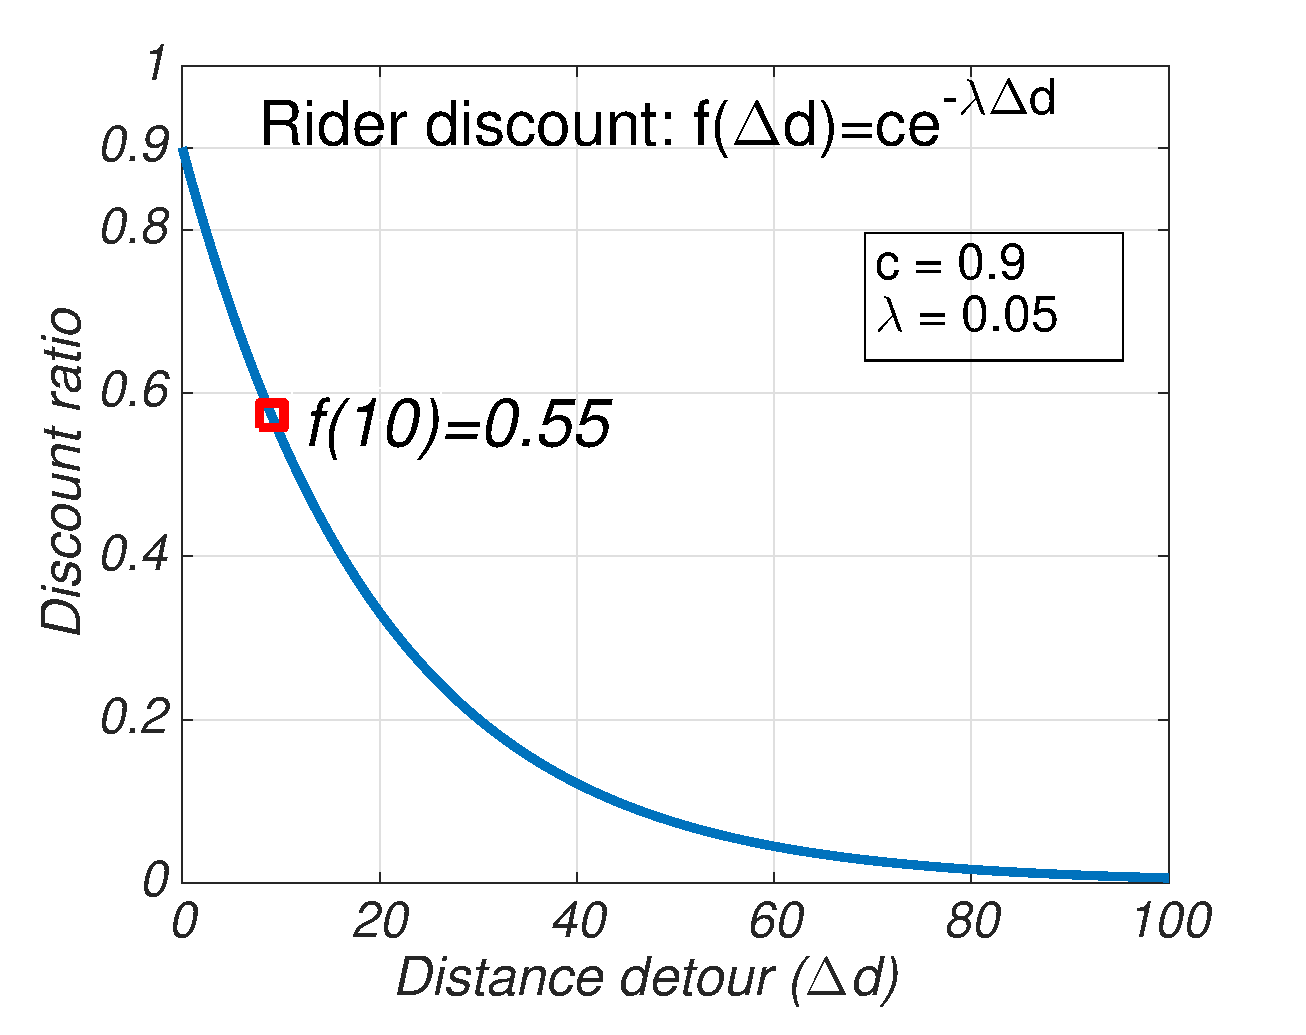
\includegraphics[width=0.45\columnwidth ]{fig/rider.eps}
    }
    \subfigure[Example Driver's Profile]{
        \label{fig:driver_profile}
        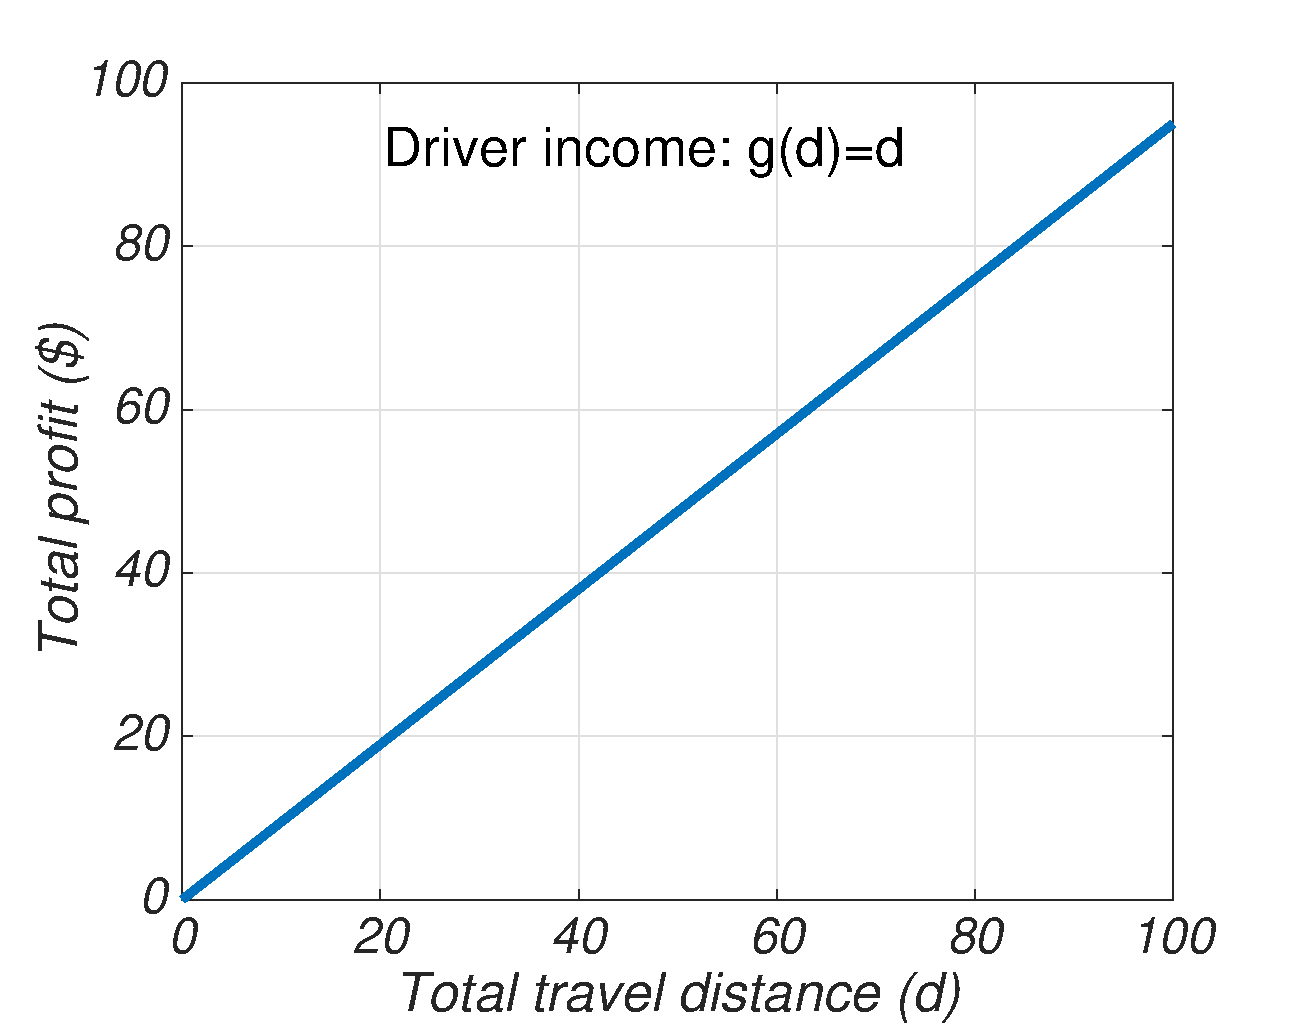
\includegraphics[width=0.45\columnwidth ]{fig/driver.eps}
    }
	\vspace{-3mm}\caption{Example User Profiles} \vspace{-2mm} \label{fig:profiles}
\end{figure}\vspace{-0mm}

Subsequently, for a request $r$ with shortest distance $d_r$, detour $\Delta d_r$ and a profile $f_r$, the final fare is represented as:
\vspace{-1.5mm}
\begin{equation}
\label{eq:fare}
fare(r) = F(d_r) f_r(\Delta d_r)
\end{equation}

\noindent This guarantees that no rider pays more than what he would have paid if he took a solo ride. In fact, the rider will get compensated for longer trips due to the detour. This satisfies the first rule of our fair pricing model.

%\subsection{Driver's Income}
Every driver has a unique profile which allows him to specify the cost of his service. Similar to riders, drivers can have different expectations for participating in ride-sharing platforms. The drivers' profile allows them to set their expectations with respect to how much they expect to be paid for participating in the platform. The driver's profile can be any function. In fact, it can take any arbitrary input in addition to the distance. For example, it is possible to define the driver's profile as $g: \mathbb{N} \times \mathbb{R}_{+}  \rightarrow \$$ where for $\left\langle n, d \right\rangle \in \mathbb{N} \times \mathbb{R}_{+}$, $n$ and $d$ are the number of passengers being serviced by the driver and the driver's total traveled distance, respectively. Without loss of generality, we assume distance is the only input of the driver's profile. Intuitively, the profile is a monotonically increasing function. For example, the profile in \cref{fig:driver_profile} is one where the driver charges \$1 per mile.

At any point in time, each driver has a schedule. A driver will be compensated during the time its schedule is not empty. Therefore, for every driver $v$, the income is:
\vspace{-2mm}
\begin{equation}
\label{eq:payment}
income_v = \int_{start_s}^{end_s} I\left( S_v(t) \neq \left\langle \right\rangle\right).g(d(t))dt
\end{equation}

\noindent Where $I()$ is the indicator function, $S_v(t)$ and $d(t)$ are the driver's schedule and the distance he travels at time $t$, respectively. In addition, $start_s$ and $end_s$ are the first pick-up time and last drop-off time of $S_v$. Consequently, regardless of the serviced requests, each driver receives an income only based on his total travel distance. This satisfies the second rule of our fair pricing model.

%\subsection{Revenue}
The amount of a driver's compensation does not necessarily have to be the same as what the riders pay for the same distance. It is the framework's responsibility to assign riders with drivers where their profiles are compatible. The profit APART makes from driver $v$ is the difference between the fares collected from all riders serviced by $v$ and the income $v$ receives for himself. Subsequently, the total profit (revenue) of APART is the sum of the profits received from all drivers:
\vspace{-3mm}
\begin{align}
\label{eq:profit} 
profit_v &= \sum_{r_i \in s_v}fare(r_i) - cost_v\\
revenue &= \sum_{v \in V}profit_v
\end{align}
\vspace{-2mm}

A price-aware framework can utilize pricing models and profiles in order to provide a better service quality. Consider the example in \cref{fig:quality_eg} where a driver is en-route to pick-up a rider from $s_1$ and drop-off at $e_1$. Before the driver reaches $s_1$ a new request arrives with $s_2$ and $e_2$ as the pick-up and drop-off locations, respectively. We also assume both $\lbrace s_1, s_2, e_1, e_2 \rbrace$ (\cref{fig:quality_sp}) and $\lbrace s_1, e_1, s_2, e_2 \rbrace$ (\cref{fig:quality_sd}) are valid schedules. Any algorithm with the objective of minimizing the total travel distance will select the route in \cref{fig:quality_sp}. With APART, the riders are able to set their profiles such that the framework might end up selecting either routes. For example, if riders want to get to their destination with the least amount of detour, they can set their expected compensation for small detours to a high value and the framework will select the route in \cref{fig:quality_sd} as the schedule for the driver. On the other hand, if riders are willing to share a ride and reduce the cost of their ride, they can do so by configuring their profiles differently. Depending on what the riders and drivers accept as a higher quality service, by setting their respected profiles they can adjust APART to provide them with a service that better suits them. Here we only considered two riders and a single driver in order to make the example in \cref{fig:quality_eg} simple. Even though in this example, a smaller detour is achieved through avoiding carpooling, in the experiments in \cref{subsec:pricingexp} we show that at least 80-90\% of the riders do engage in carpooling and yet, end up with a detour of only 6-7\% of their original trip.

\begin{figure}[!ht]
	\centering
    \subfigure[\scriptsize{Minimize Driver's Distance}]{
        \label{fig:quality_sp}
        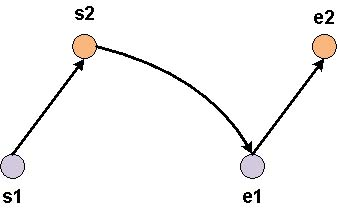
\includegraphics[width=0.4\columnwidth ]{fig/quality_eg_sp.jpg}
    }
    \subfigure[\scriptsize{Minimize Rider's Detour}]{
        \label{fig:quality_sd}
        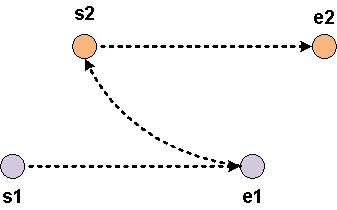
\includegraphics[width=0.4\columnwidth ]{fig/quality_eg_sd.jpg}
    }
	\vspace{-2mm}\caption{Examply of Price-aware Scheduling} \vspace{-2mm} \label{fig:quality_eg}
\end{figure}\vspace{-0mm}

We end this section with a note on the versatility of our pricing model. We explained our pricing model based on the objective of our framework which is maximizing the provider's revenue. However, using the same definitions and by configuring the riders' and drivers' profiles differently, we can adjust the framework to achieve other objectives as well. For example, consider minimizing total travel distance of drivers. Many studies \cite{Ma13,Huang14,Ma15} achieve this goal by assigning a new request to the driver with the least increase in travel distance. \cref{th:min_dist} shows, with only configuring the riders' and drivers' profiles appropriately, APART can make exactly the same assignments and achieve the same objective.

\vspace{-2mm}
\begin{theorem}
\label{th:min_dist}
If all the riders' profiles are set to $f'_r = 1$ and every drivers' profiles to $g'_v = 1$, by selecting the most profitable driver, APART will select the driver with the minimum increase in travel distance.
\end{theorem}

\begin{proof}
Upon arrival of a new request $r$, each driver in APART finds a schedule which generates the most profit. Since $f'_r(\Delta d_r) = 1$, regardless of $\Delta d_r$, the final fare for $r$ is equal to $F(d_r)$ where $d_r$ is the length of the shortest path between $r$'s pick-up and drop-off points. Therefore, for an incoming request $r$, every driver $v$ can compute the maximum profit it can generate for the system upon accepting $r$ as: $profit_v = F(d_r) - g'(\Delta d_v)$ where $\Delta d_v$ is the increase in $v$'s traveled distance if $r$ is assigned to $v$. Since $F(d_r)$ is the same regardless of the driver, the most profitable driver is the one with the smallest $\Delta d_v$.
\end{proof}